\documentclass{article}[12pt,a4paper]
\usepackage[utf8]{inputenc}
\usepackage{caption}
\usepackage{amsmath} 
\usepackage{hyperref}
\usepackage{csquotes}
\usepackage{graphicx}

\hypersetup{
    colorlinks=true,
    linkcolor=blue,
    filecolor=magenta,      
    urlcolor=cyan,
}

\title{For Whom The Kettlebell Tolls}
\author{Rátki Barnabás}
\date{2020.08.10}

\begin{document}
\maketitle

A feladat a következő volt: \begin{displayquote}
Beküldendő az emelőrendszerek áttétele az ábra alapján (tehát az egységnyi, "kézben tartott” erőnél hányszor nehezebb a kettlebell). Ahol masni van, az fix kötést jelent kötél-kötél vagy kötél-kettlebell között. (3 pont)
\end{displayquote}

\section{Megoldás}
Egy módszer egy ilyen rendszerben az áttétel meghatározásának a "T-method" vagy "tension method", az a lényege, hogy amikor a kötél átmegy egy csigán, a "feszülése" ugyan az marad. Illetve amikor két kötél rész tart egy harmadik részt, akkor azt a kettő rész össz "feszülésével" teszik.

Ezek alapján az ábrákat felcímkéztem, az adott kötélszakaszban lévő "feszülés" szerint, végeredményében ez azt foglya jelenti, hogy a bemeneti kötélszállon (ahol húzzuk), erőnk annyival "sokszorozódik" meg mint ami a súlyon lévő szám lesz.

A feladatban azt is feltételezzük, hogy a kötél súlytalan, minde csiga ideális, nincsen semmilyen közegellenállás, vagy surlódás vagy veszteség sehol.

\section{Első rendszer}
\begin{center}
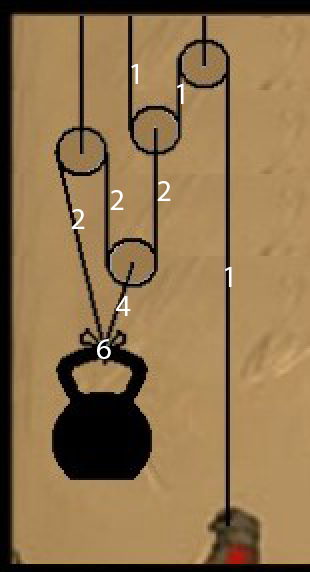
\includegraphics[scale=0.5]{1kettle}
\end{center}
Itt tehát az áttétel 6-os ezért, a kettlebell 6x nehezbb mint az erő amivel tartani kell.

\section{Második rendszer}
\begin{center}
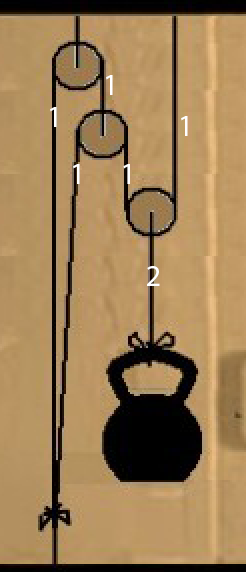
\includegraphics[scale=0.5]{2kettle}
\end{center}
Kétszer nehezebb a kettlebell mint az erő amivel tartani kell.

\section{Harmadik rendszer}
\begin{center}
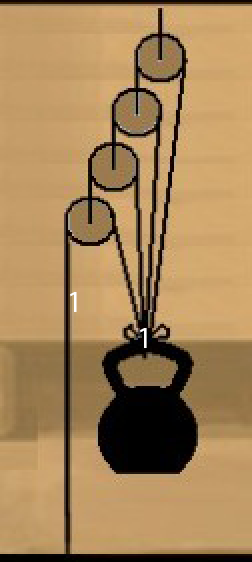
\includegraphics[scale=0.5]{3kettle}
\end{center}
A kettlebell ugyan olyan nehéz mint ahogyan tartani kell, csupán az kifejtendő erő irányát változtattuk meg.

\section{Negyedik rendszer}
\begin{center}
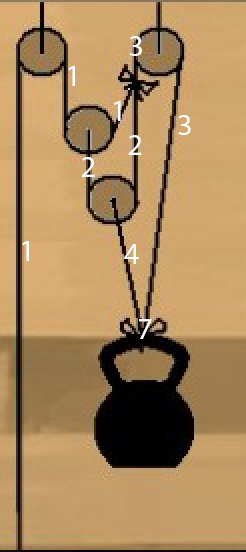
\includegraphics[scale=0.5]{4kettle}
\end{center}
A kettlebell 7x nehezebb mint az erő amivel tartani kell.


\end{document}
